
\begin{figure*}[ht]
\begin{center}
	\rule{1\linewidth}{0pt}
        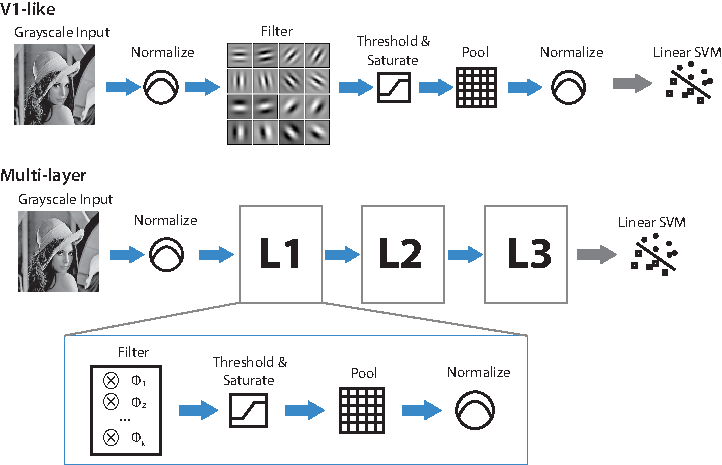
\includegraphics[width=1\linewidth]{figures/models_v2.pdf}
\end{center}
   \caption{{\bf A schematic diagram of the system architecture of the family of
       models considered.}  Each model consists of one to three feedforward
     filtering layers, with the filters in each layer being applied across the
     previous layer.}
\label{fig:models}
\end{figure*}



% -----------------------------------------------------------------------------
\subsection{Large-scale feature search framework}
% -----------------------------------------------------------------------------
\label{sec:feature_search}

The large-scale feature search approach used here consists of four basic components:
(1) a parametric family of feature representation, wherein key aspects of the behavior of the 
features are controlled by a fixed set of parameters, (2) a generation procedure for 
choosing models from the larger family to evaluate, (3) a screening procedure, run on 
each candidate feature representation, to determine which models to evaluate further
and (4) a validation procedure, using independent data, to evaluate the utility of representations found
during the screening procedure.

The approach we follow here is similar to that described in \cite{pinto:plos09},
with two important differences, which we describe briefly here, and detail in depth below.
First, Pinto et al. \cite{pinto:plos09} used an unsupervised learning procedure in 
order to learn certain model parameters from a pre-training video set.  Here, we dispense with 
this unsupervised learning procedure, instead opting for greatly speeded model generation, allowing
more model architectures to be evaluated per unit time.  Second, we used the \emph{LFW View 1} subset 
as a screening set.  Details of the model family considered, and generation, screening and validation  
procedures used are described below.


% -----------------------------------------------------------------------------
\subsection{Biologically-inspired visual representations}
% -----------------------------------------------------------------------------
\label{sec:models}

In our experiments, we used two basic classes of biologically-inspired visual 
representations, shown in Fig.
\ref{fig:models}. 

First, as a  control, we used \emph{V1-like}, a 
one-layer model characterized by a
cascade of linear and nonlinear processing steps and designed to encapsulate
some of the known properties of the first cortical processing stage in the
primate brain.  Our \emph{V1-like} implementation was taken without modification from
\cite{pinto:plos08,pinto:eccv08}.

Second, we used two and three layer models following the basic multi-layer model
scheme described in \cite{pinto:plos09}.  Briefly, these
models consist of multiple stacked layers of linear-nonlinear processing stages,
similar to those in the \emph{V1-like} model.  Importantly, in order to speed the
processing of these models, we disabled the unsupervised learning mechanisms described in
\cite{pinto:plos09} and instead used \emph{random} filter kernels drawn from a uniform
distribution.  Prior experience of our group and others \cite{jarrett-iccv-09}
has suggested that random filters can in many cases function surprisingly well
for models belonging to this general class. Details of each model class follow.


\subsection{``V1-like'' visual representation}

In the \emph{V1-like} representation, features were taken without additional
optimization from Pinto et al.'s \emph{V1S+} \cite{pinto:plos08}.  This visual
representation is based on a first-order description of primary visual cortex V1
and consists of a collection of locally-normalized, thresholded Gabor wavelet
functions spanning a range of orientations and spatial frequencies.

% \emph{V1-like} features have been proposed by neuroscientists as a ``null''
% model (a baseline against which performance can be compared) for object and face
% recognition since they do not contain a particularly sophisticated
% representation of shape or appearance, nor do they possess any explicit
% mechanism designed to tolerate image variation (e.g. changes in view, lighting,
% position, etc. \cite{dicarlo:tics07,pinto:plos08}). Here, this model serves as
% a lower bound on the level of performance that can be achieved by only relying
% on relatively low-level regularities that exist in the test set.  To be
% considered a promising face recognition system in unconstrained settings, a
% model should minimally exceed the performance of the \emph{V1-like} model.

In spite of their simplicity, these features have been shown to be among the
best-performing non-blended features set on standard natural face and object
recognition benchmarks \cite{pinto:plos08,pinto:eccv08,pinto:cvpr09} (i.e. \emph{Caltech-101}\cite{feifei2007lgv},
\emph{Caltech-256}\cite{caltech256}, \emph{ORL}\cite{orl},
\emph{Yale}\cite{yale}, \emph{CVL}\cite{cvl}, \emph{AR}\cite{ar}, \emph{LFW}\cite{huang:lfw}) and are a key component of the
best blended solutions for some of these same benchmarks
\cite{gehler:iccv09}. We used the authors' publicly available source code to
generate these features and followed the same basic read-out/classification
procedure as detailed in \cite{pinto:plos08}, with two minor modifications.
Specifically, no PCA dimensionality reduction was performed prior to
classification (the full vector was used), and a different SVM regularization
parameter was used ($C=10^5$ instead of $C=10$, see below).

For a detailed description of the \emph{V1-like} visual representation, we refer
the interested reader to the methods of the original publication
\cite{pinto:plos08} and its source code.


\subsection{High-throughput-derived multilayer visual representations: \emph{HT-L2} and \emph{HT-L3}}

% In this study, we considered the five best two- and three-layer models generated
% from a high-throughput feature search procedure (model selection) for a total of 10
% multilayer visual representations.  An important feature of the generation of
% these representations, according to the basic scheme set forth in \cite{pinto:plos09},
% is the use of a massively parallel, high-throughput search over the parameter
% space of all possible instances of a large class of biologically-inspired
% models. Details of this model class and the high-throughput screening (model
% selection) procedure are modified from \cite{pinto:plos09} and are described below.

% --------------------------------------
\subsubsection{Model architecture: }

Candidate models were composed of a hierarchy of two (\emph{HT-L2}) or three
layers (\emph{HT-L3}), with each layer including a cascade of linear and
nonlinear operations that produce successively elaborated nonlinear feature-map
representations of the original image. A diagram detailing the flow of
operations is shown in Fig. \ref{fig:models}, and, for the purposes of notation,
the cascade of operations is represented as follows:

\begin{align*}
Layer^{0}: &\\ &\mathbf{Input}
\buildrel{\mathbf{Grayscale}}\over{\longrightarrow} \mathbf{ }
\buildrel{\mathbf{Normalize}}\over{\longrightarrow} \mathbf{N^{0}} %\\ Layer^{1}:
% &\\ &\mathbf{N^{0}} \buildrel{\mathbf{Filter}}\over{\longrightarrow}
% \mathbf{F^{1}} \buildrel{\mathbf{Activate}}\over{\longrightarrow} \mathbf{A^{1}}
% \buildrel{\mathbf{Pool}}\over{\longrightarrow} \mathbf{P^{1}}
% \buildrel{\mathbf{Normalize}}\over{\longrightarrow} \mathbf{N^{1}}
\end{align*}

and generally, for all $\ell \ge 1$:
\begin{align*}
Layer^{\ell}: &\\ &\mathbf{N^{\ell - 1}}
\buildrel{\mathbf{Filter}}\over{\longrightarrow} \mathbf{F^{\ell}}
\buildrel{\mathbf{Activate}}\over{\longrightarrow} \mathbf{A^{\ell}}
\buildrel{\mathbf{Pool}}\over{\longrightarrow} \mathbf{P^{\ell}}
\buildrel{\mathbf{Normalize}}\over{\longrightarrow} \mathbf{N^{\ell}}
\end{align*}

Details of these steps along with the range of parameter values included in the
random search space are described next.

% --------------------------------------
\subsubsection{Input and Pre-processing}

The input of the \emph{HT-L2} and \emph{HT-L3} models were 100x100 and 200x200
pixel images, respectively. In the pre-processing stage, referred to as
$Layer^{0}$, this input was converted to grayscale and locally normalized:

\begin{equation}\label{eq:input}
\mathbf{N^{0}=Normalize(Grayscale(Input))}
\end{equation}
where the $\mathbf{Normalize}$ operation is described in detail below.  Because
this normalization is the final operation of each layer, in the following
sections, we refer to $N^{\ell-1}$ as the input of each $Layer^{\ell>0}$ and
$N^{\ell}$ as the output.


% --------------------------------------
\subsubsection{Linear Filtering}

%\paragraph{ }
%\emph{Description:}
The input $N^{\ell-1}$ of each subsequent layer (i.e.  $Layer^{\ell}, \ell \in
\{1,2,3\}$) was first linearly filtered using a bank of $k^{\ell}$ filters to
produce a stack of $k^{\ell}$ feature maps, denoted $F^{\ell}$.  In a
biologically-inspired context, this operation is analogous to the weighted
integration of synaptic inputs, where each filter in the filterbank represents a
different cell.

%\emph{Definitions:}
The filtering operation for $Layer^{\ell}$ is denoted:
\begin{equation}
    \mathbf{F^{\ell} = Filter(N^{\ell-1}, \Phi^{\ell})}
\end{equation}
and produces a stack, $F^{\ell}$, of $k^{\ell}$ feature maps, with each map,
$F_{i}^{\ell}$, given by:
\begin{equation}\label{eq:filter}	
%F^{\ell}_i = N^{\ell-1} \otimes \Phi^{\ell}_i \qquad \forall i \in \{
F^{\ell}_i = N^{\ell-1} \otimes \Phi^{\ell}_i \quad \forall i \in \{
1,2,\dotsc,k^{\ell} \}
\end{equation}
where $\otimes$ denotes a correlation of the output of the previous layer,
$N^{\ell-1}$ with the filter $\Phi^{\ell}_i$ (e.g. sliding along the first and
second dimensions of $N^{\ell-1}$).  Because each successive layer after
$Layer^{0}$ is based on a stack of feature maps, $N^{\ell-1}$ is itself a stack
of 2-dimensional feature maps.  Thus, the filters contained within $\Phi^{\ell}$
are, in turn, 3-dimensional, with the their third dimension matching the number
of filters (and therefore, the number of feature maps) from the previous layer
(i.e. $k^{\ell-1}$).

%\paragraph{ }
\emph{Parameters:}
\begin{itemize}
\item The filter shapes ${f_s}^{\ell} \times {f_s}^{\ell} \times {f_d}^{\ell}$
  were chosen randomly with ${f_s}^{\ell} \in \{3, 5, 7, 9\}$ and
  ${f_d}^{\ell}=k^{\ell-1}$.
\item Depending on the layer $\ell$ considered, the number of filters $k^{\ell}$
  was chosen randomly from the following sets:
\begin{itemize}
\item In $Layer^{1}$, $k^{1} \in \{16, 32, 64\}$
\item In $Layer^{2}$, $k^{2} \in \{16, 32, 64, 128\}$
\item In $Layer^{3}$, $k^{3} \in \{16, 32, 64, 128, 256\}$
\end{itemize}
\end{itemize}
All filter kernels were fixed to random values drawn from a uniform
distribution.


% --------------------------------------
\subsubsection{Activation Function}

%\paragraph{ }
%\emph{Description:}
Filter outputs were subjected to threshold and saturation activation function,
wherein output values were clipped to be within a parametrically defined range.
This operation is analogous to the spontaneous activity thresholds and firing
saturation levels observed in biological neurons.

%\paragraph{ }
%\emph{Definitions:}
We define the activation function:
\begin{equation}
\mathbf{A^{\ell} = Activate(F^{\ell})}
\end{equation}
that clips the outputs of the filtering step, such that:
\begin{equation}\label{eq:activ}
	\mathbf{Activate(x)} = \left\{
	\begin{array}{ll}
		{\gamma_{max}}^{\ell} & \mbox{if $x >
                  {\gamma_{max}}^{\ell}$}\\ {\gamma_{min}}^{\ell} & \mbox{if $x
                  < {\gamma_{min}}^{\ell}$}\\ x& \mbox{otherwise}
	\end{array}
	\right.
\end{equation} 
Where the two parameters ${\gamma_{min}}^{\ell}$ and ${\gamma_{max}}^{\ell}$
control the threshold and saturation, respectively.  Note that if both minimum
and maximum threshold values are $-\infty$ and $+\infty$, the activation is
linear (no output is clipped).

%\paragraph{ }
\emph{Parameters:}
\begin{itemize}
\item ${\gamma_{min}}^{\ell}$ was randomly chosen to be $-\infty$ or $0$
\item ${\gamma_{max}}^{\ell}$ was randomly chosen to be $1$ or $+\infty$
\end{itemize}

\begin{figure*}[ht]
\begin{center}
	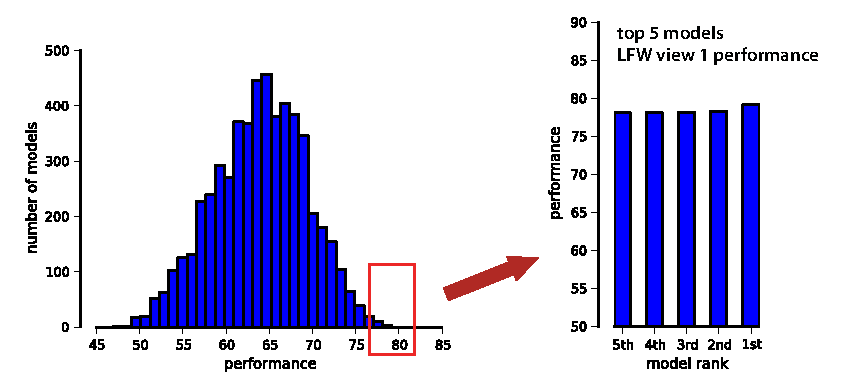
\includegraphics[scale=1]{figures/ht_process_l3.pdf}

    \caption[]{{\bf The high-throughput screening process used to find good representations.}  Here, data is shown for the screening of
      \emph{HT-L3} models.  A distribution of the performance of 6,917 randomly
      generated models is shown on the left, with the top five high-performing
      models replotted on the right.  Following screening, the models were evaluated
      exclusively with sets that do not overlap with the screening set.}

    \label{fig:ht_process}
 \end{center}
\end{figure*}


% --------------------------------------
\subsubsection{Pooling}

%\paragraph{ }
%\emph{Description:}
The activations of each filter within some neighboring region were then pooled
together and the resulting outputs were spatially downsampled.

%\paragraph{ }
%\emph{Definitions:}
We define the pooling function:
\begin{equation}
\mathbf{P^{\ell} = Pool(A^{\ell})}
\end{equation}
such that: \\
\begin{equation}\label{eq:pool}
\mathbf{P^{\ell}_{i}} = \mathbf{Downsample_{\alpha}}(
        \sqrt[p^{\ell}]{(A^{\ell}_i)^{p^{\ell}} \odot \mathbf{1}_{a^{\ell}
            \times a^{\ell}}} )
\end{equation}
, where $\odot$ is the 2-dimensional correlation function with
$\mathbf{1}_{a^{\ell} \times a^{\ell}}$ being an $a^{\ell} \times a^{\ell}$
matrix of ones ($a^{\ell}$ can be seen as the size of the pooling
``neighborhood'').  The variable $p^{\ell}$ controls the exponents in the
pooling function.

%\paragraph{ }
\emph{Parameters:}
\begin{itemize}
\item The stride parameter $\alpha$ was fixed to 2, resulting in a downsampling
  factor of 4.
\item The size of the neighborhood $a^{\ell}$ was randomly chosen from
  $\{3,5,7,9\}$.
\item The exponent $p^{\ell}$ was randomly chosen from $\{1, 2, 10\}$.
\end{itemize}
Note that for $p^{\ell}=1$, this is equivalent to blurring with a $a^{\ell}
\times a^{\ell}$ boxcar filter.  When $p^{\ell}=2$ or $p^{\ell}=10$ the output
is the $L^{p^{\ell}}$-norm
\footnote{The $L^{10}$-norm produces outputs similar to a \emph{max} operation
  (i.e. \emph{softmax}).}.



% --------------------------------------
\subsubsection{Normalization}

%\paragraph{ }
%\emph{Description:} 
As a final stage of processing within each layer, the output of the Pooling step
was normalized by the activity of their neighbors within some radius (across
space and across feature maps).  Specifically, each response was divided by the
magnitude of the vector of neighboring values if above a given threshold.  This
operation draws biological inspiration from the competitive interactions
observed in natural neuronal systems (e.g. contrast gain control mechanisms in
cortical area V1, and elsewhere \cite{geisler1992cni,rolls2002cnv})


%\paragraph{ }
%\emph{Definitions:}
We define the normalization function: 
\begin{equation}
\mathbf{N^{\ell} = Normalize(P^{\ell})}
\end{equation}
such that:
\begin{equation}\label{eq:norm}
N^{\ell} = \left\{ \scriptsize{
\begin{array}{ll}
  \rho^{\ell} \cdot C^{\ell} & \mbox{ if $ \rho^{\ell} \cdot
    \vectornorm{C^{\ell} \otimes \mathbf{1}_{b^{\ell} \times b^{\ell} \times
        k^{\ell}}}_2 < \tau^{\ell}$} \\ \frac{C^{\ell}}{\vectornorm{C^{\ell}
      \otimes \mathbf{1}_{b^{\ell} \times b^{\ell} \times k^{\ell}}}_2} &
  \mbox{otherwise}
\end{array}
} \right.
\end{equation}
with
\begin{equation}
C^{\ell} = P^{\ell}-\delta^{\ell} \cdot \frac{P^{\ell} \otimes
  \mathbf{1}_{b^{\ell} \times b^{\ell} \times k^{\ell}}}{b^{\ell} \cdot b^{\ell}
  \cdot k^{\ell}}
\end{equation}
Where $\delta^{\ell} \in \{0,1\}$, $\otimes$ is a 3-dimensional correlation over
the ``valid'' domain (i.e. sliding over the first two dimensions only), and
$\mathbf{1}_{b^{\ell} \times b^{\ell} \times k^{\ell}}$ is a $b^{\ell} \times
b^{\ell} \times k^{\ell}$ array full of ones.  $b^{\ell}$ can be seen as the
normalization ``neighborhood'' and $\delta^{\ell}$ controls if this neighborhood
is centered (i.e. subtracting the mean of the vector of neighboring values)
before divisive normalization.  $\rho^{\ell}$ is a ``magnitude gain'' parameter
and $\tau^{\ell}$ is a threshold parameter below which no divisive normalization
occurs.

%\paragraph{ }
\emph{Parameters:}
\begin{itemize}
\item The size $b^{\ell}$ of the neighborhood region was randomly chosen from
  $\{3,5,7,9\}$.
\item The $\delta^{\ell}$ parameter was chosen from $\{0,1\}$.
\item The vector of neighboring values could also be stretched by gain values
  $\rho^{\ell} \in \{10^{-1}, 10^{0}, 10^{1}\}$. Note that when $\rho^{\ell} =
  10^{0} = 1$, no gain is applied.
\item The threshold value $\tau^{\ell}$ was randomly chosen from $\{10^{-1},
  10^{0}, 10^{1}\}$.
\end{itemize}

% --------------------------------------
\subsection{Final model output dimensionality}
\label{sec:final_dim}

The output dimensionality of each candidate model was determined by the number
of filters in the final layer, and the x-y ``footprint'' of the layer (which, in
turn, depends on the subsampling at each previous layer).  In the model space
explored here, the possible output dimensionality ranged from 256 to 73,984.

% min = 256 = 1x1x256
% max = 73984 = 17x17x256 
% ( (((((((input-norm0-filt1-pool1)/2)-norm1-filt2-pool2)/2)-norm2-filt3-pool3)/2)-norm3) 
% = (((((((200-2-2-2)/2)-2-2-2)/2)-2-2-2)/2)-2) = 17)

% --------------------------------------
\subsection{Screening (model selection)}

A total of 5,915 \emph{HT-L2} and 6,917 \emph{HT-L3} models were screened on the \emph{LFW}
View 1 ``aligned'' set \cite{taigman:bmvc09}.  We selected the best five models
from each ``pool'' for further analysis on the \emph{LFW} View 2 set (Restricted
Protocol).  Note that \emph{LFW} View 1 and View 2 do not contain the same
individuals and are thus mutually exclusive sets. View 1 was designed as a model
selection set while View 2 is used as an independent validation set for the
purpose of comparing different methods.

Examples of the screening procedure for \emph{HT-L2} and \emph{HT-L3} models on the
\emph{LFW} View 1 task screening task are shown in Fig. \ref{fig:ht_process}.
Performance of randomly generated \emph{HT-L3} models ranged from chance performance
(50\%) to better than 80\% correct; the best five models were drawn from this
set and are denoted \emph{HT-L3-1st}, \emph{HT-L3-2nd}, and so on.  An analogous
procedure was undertaken to generate five two-layer models, denoted
\emph{HT-L2-1st}, \emph{HT-L2-2nd}, etc.



% --------------------------------------
\subsection{Evaluation Protocol}

To evaluate the performance of our biologically-inspired
representations, we followed the standard \emph{LFW} face verification
``Restricted View 2'' protocol.  6,000 different face image pairs (half
``same'', half ``different'') were drawn randomly from the sets and divided into
10-fold cross validation splits with 5,400 training and 600 testing examples
each.

Because the biologically-inspired representations used here generate one feature
vector per image, comparison functions were used to generate a new feature
vector for each pair, and these ``comparison'' features were used to train
binary (``same'' / ``different'') hard-margin linear SVM classifiers.  Following
\cite{pinto:cvpr09} we used the following element-wise comparison functions:
$|F_1 - F_2|$, $\sqrt{|F_1 - F_2|}$, $(F_1 - F_2)^2$, where $F_1$ and $F_2$
are the feature vectors generated from the first and the second image of the
pair, respectively.  We additionally added the comparison function $(F_1 \cdot
F_2)$, which was not used in \cite{pinto:cvpr09}, under the logic that it serves
as a soft ``AND''-like function (i.e.  it primarily results in a large response
for elements where both $F_1$ and $F_2$ are large). We hypothesized that such a
function would be valuable since our representations are all quite sparse, and
thus a coincidence of high feature values in common between the two test images
is likely to provide meaningful evidence of similarity.



\subsection{Kernel combinations and data-set augmentation}

While the high-throughput search techniques described above are capable of
yielding relatively high-performing individual representations for \emph{LFW} by
themselves, effectively all of the top-performing face recognition systems on
\emph{LFW} employ some form of more advanced machine learning backend to enhance
their performance \cite{taigman:bmvc09,wolf:accv09,kumar:iccv09,cao2010face}.  One common approach in this
regard is to blend together a large number of weak learners to produce
a blended classifier.

To explore what performance enhancement can be gained with modest amounts of
blending on top of our feature representations, we pursued a progressive strategy
of layering on additional kernels to produce successively larger and higher
performing blends. Two basic strategies were used for generating new kernels: 1)
feature augmentation, performing operations on the input image, such as cropping
and rescaling to produce alternate kernels using the same representation, and 2)
representation blending, that is, combining together kernels derived from
multiple separate feature representations (e.g. blending over the five
\emph{HT-L2} top models, or combining the top five \emph{HT-L2} and \emph{HT-L3}
models).

The progression of these additional elaborations is described below:

\subsubsection{Multiple rescaled crops}

Following \cite{pinto:cvpr09}, we augmented the dataset by computing features on
three different centered crops of the image: 250x250 (original), 150x150 and
125x75.  Each of these crops was resized to the standard input size of each representation,
and SVMs were trained separately for each crop size.
Blending of the resulting kernels was done by simple kernel addition, with each
kernel being trace-normalized (by the training kernel trace) prior to summation.
More sophisticated blending (e.g. IKL/MKL\cite{sonnenburg2006lsm},
LP-Boost\cite{gehler:iccv09}) were not used at this stage.

\subsubsection{Blending of the top 5 models within class}

While the top five models found by our high-throughput search all yield similar
levels of performance, they achieve this performance with different parameter
sets.  Consequently, to the extent that the top five models represent a
diversity of different ways to achieve good performance, we would expect that
blending these models would yield further enhancement of performance.  At this
stage, we combined all of the Stage 1 kernels above (multiple rescaled crops) from each of the top five
models within each model-class (e.g. \emph{HT-L2} and \emph{HT-L3}).

\subsubsection {Hierarchical blends across model class}

Finally, we also explored a more principled way to blend the representations
from each model class.  Following \cite{phow} we assigned exponentially larger
weight to higher-level representation (\emph{V1-like} $<$ \emph{HT-L2} $<$
\emph{HT-L3}) resulting in the following kernel: 

\begin{equation}
K(\cdot,\cdot) =
\displaystyle\sum_{\ell} (2^{\ell-1}) k_{\ell}(\cdot, \cdot)
\end{equation}

where $\ell=1$ for
\emph{V1-like} (one layer), $\ell=2$ for the top five \emph{HT-L2} (two layers)
and $\ell=3$ for the top five \emph{HT-L3} (three layers).

We note that the choice of blending strategies to consider on the View 2 set was 
driven by performance on the View 1 set, thereby avoiding selection bias artifacts.

\subsection{Additional Testing with Synthetic Face Images}

In order to assess model performance on an image set with a known amount of variation, 
we generated a set of 3D-rendered face images.  3D face meshes were randomly generated
using the FaceGen software package and were rendered using
the free POV-Ray ray-tracer.  For each rendered image, a model rotation 
(azimuth and elevation), position (x and y), and scale were drawn from a uniform 
distribution and the models were rendered with a common light source (Figure \ref{fig:variation_levels}).  
For the experiments presented here, rotation, size, and position were combined into
a single composite ``variation level'' wherein the variation in the pixel-level euclidean norm
was equalized for each kind of variation (e.g. one ``unit'' of rotation variation produced an
equivalent pixel-level change as one ``unit'' of position variation).  Examples of several
variation ``levels'' are shown in Figure \ref{fig:variation_levels}.

The rendered face/head was next composited onto one of four kinds of backgrounds: no
background, a white noise background, a phase-scrambled natural background 
(approximately equivalent to 1/f noise), and a randomly chosen natural background, chosen from
a large pool of outdoor background images (Figure \ref{fig:bg_variation}).  Care was taken 
to ensure that the same background image was never used in more than one final image.

\begin{figure*}[ht]
\centering 
\subfigure[\small{View, position an scale variation}]{
  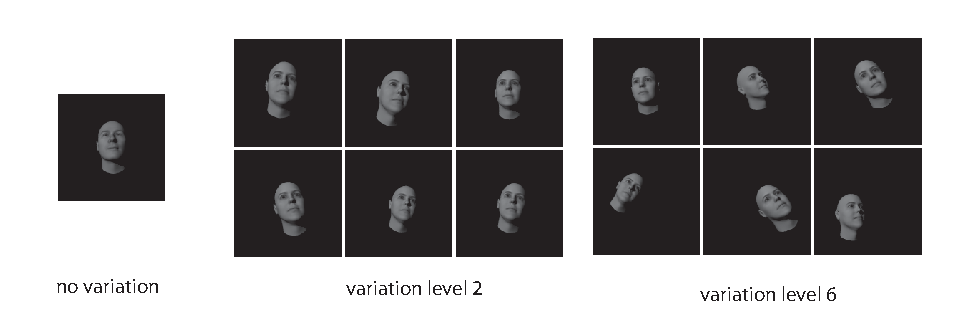
\includegraphics[scale=0.8]{figures/nongenerated/variation_level.pdf}
  \label{fig:variation_levels}
} 
\subfigure[\small{Background variation}]{
  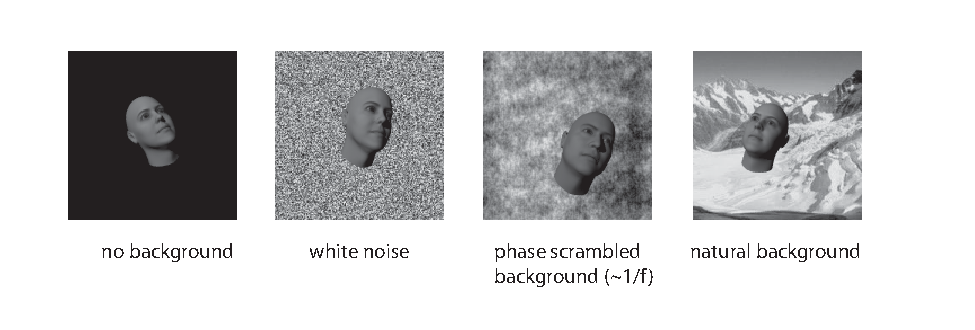
\includegraphics[scale=0.8]{figures/nongenerated/bg_variation.pdf}
  \label{fig:bg_variation}
} 
\caption[]{{\bf Synthetic face stimuli}}
\label{fig:synthetic_faces}
\end{figure*}
